\section{Filter-Theorie}
\subsection{Nomogramm}
\script{393} Mittels Stempel und Matrix können die Ordnung von Filtern durch das Nomogramm berechnet werden. Nach folgenden Punkten kann $P_5$ für den nächst höheren gelegene Kurve ($n$) gefunden werden.
\begin{center}
	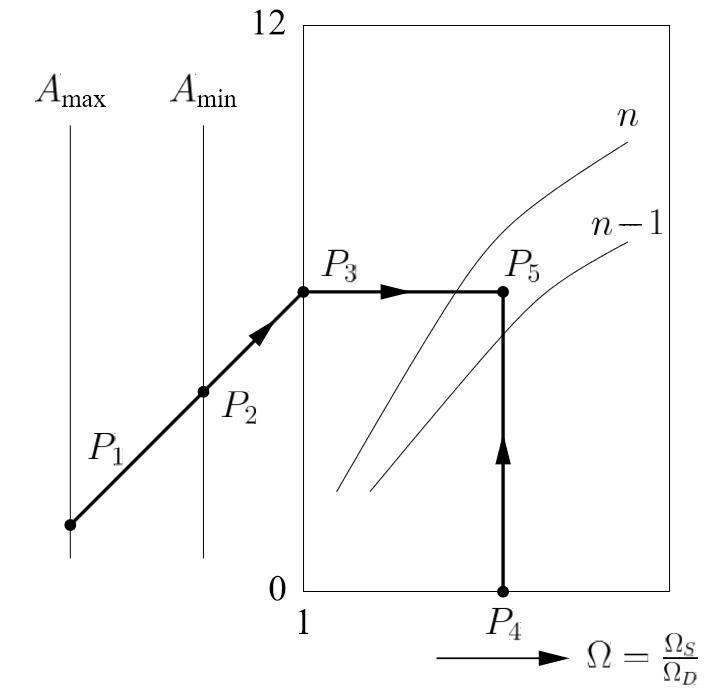
\includegraphics[width=0.6\columnwidth]{Images/nomogramm}
\end{center}
Für Gleichungen siehe \script{394}